\documentclass{beamer}
\usepackage{beamerthemeshadow}
\usepackage{verbatim}

\usepackage{lastpage}
\usepackage{xcolor}
\usepackage{pgf}
\usepackage{colortbl}
\usepackage{hyperref}
\usepackage{multirow}
\usepackage{dsfont}
\usepackage{graphbox}


\usepackage{siunitx}
\sisetup{input-symbols=(), group-digits  = false} 

\newcommand{\bi}{\begin{itemize}}
\newcommand{\ei}{\end{itemize}}
\newcommand{\be}{\begin{enumerate}}
\newcommand{\ee}{\end{enumerate}}
\newcommand{\bd}{\begin{description}}
\newcommand{\ed}{\end{description}}
\newcommand{\prbf}[1]{\textbf{#1}}
\newcommand{\prit}[1]{\textit{#1}}
\newcommand{\beq}{\begin{equation}}
\newcommand{\eeq}{\end{equation}}
\newcommand{\bdm}{\begin{displaymath}}
\newcommand{\edm}{\end{displaymath}}

\newcommand{\ft}[1]{
  \frametitle{\begin{tabular}{p{4.2in}r} \textcolor{white}{#1} & \small{\insertframenumber / \inserttotalframenumber} \end{tabular}}
  \setbeamercovered{transparent=18}
}

\newcommand{\eft}[1]{
  \frametitle{\begin{tabular}{p{4in}r} \textcolor{white}{#1} & \small{\hyperlink{f:questions}{\beamergotobutton{GO BACK}}} \end{tabular}}
  \setbeamercovered{transparent=18}
}

\newcommand{\stepinv}{\setbeamercovered{invisible}}
\newcommand{\stopinv}{\setbeamercovered{transparent=18}}
\newcommand{\uncoverinv}[1]
{
  \setbeamercovered{invisible}
  \uncover<+->{#1}
  \setbeamercovered{transparent=18}
}
\newcommand{\ans}[1]{\textcolor{blue}{#1}}
\newcommand{\ansinv}[1]
{
  \setbeamercovered{invisible}
  \uncover<+->{\textcolor{blue}{#1}}
  \setbeamercovered{transparent=18}
}
\newcommand{\setinv}{\setbeamercovered{invisible}}
\newcommand{\setvis}{\setbeamercovered{transparent=18}}
\newcommand{\centerpic}[2]
{
  \begin{center}
  \includegraphics[#1]{#2}
  \end{center}
}
\newcommand{\h}[1]{\hat{#1}}
\newcommand{\ds}{\displaystyle}

\definecolor{light}{rgb}{1.0,0.7,0.7}
\definecolor{BrickRed}{rgb}{0.8,0.1,0.1}
%\definecolor{light}{rgb}{1.0,0.5,0.5}
%\newcommand{\hl}[1]{\only<#1>{\cellcolor{BrickRed}}}
\newcommand{\hl}[1]{\textcolor<#1>{BrickRed}}

\definecolor{mycolor}{rgb}{0.6,0.0,0.0}
\usecolortheme[named=mycolor]{structure}

\title[Regime Switching in Fiscal Policy functions]{Regime Switching in Fiscal Debt Targets and Policy Functions in the United States}
\author[James M. Murray, University of Wisconsin - La Crosse]
{
James M. Murray, Ph.D.\\
Department of Economics\\
University of Wisconsin - La Crosse
}
\date{November 17, 2017}

\begin{document}

\frame{\titlepage \setcounter{framenumber}{0}}

\begin{frame}
  \ft{Purpose}
  \uncover<+-> {
  \begin{block}{Describe fiscal policy dynamics}
    \begin{tabular}{ll}
    Government expenditures & Deficits \\
    Income tax rate & Debt \\
    Net transfer payments
    \end{tabular}
  \end{block}
  } % end uncover

  \uncover<+->{
  \begin{block}{Describe debt service}
    \begin{enumerate}
    \item How do these fiscal policy variables respond to \textit{debt / GDP}?
    \item What is the implied target for \textit{debt / GDP}?
    \item Is there switching in these fiscal policy responses?
    \item Is there switching in the long-run debt target?
    \end{enumerate}
  \end{block}
  } % end uncover

  \uncover<+->{
  \begin{block}{Describe stabilizing behavior}
    \begin{enumerate}
    \item How do fiscal policy variables respond to \textit{output gap}?
    \item Is there switching in these fiscal policy responses?
    \end{enumerate}
  \end{block}
  } % end uncover
\end{frame}

\begin{frame}
  \ft{Fiscal Variables}
  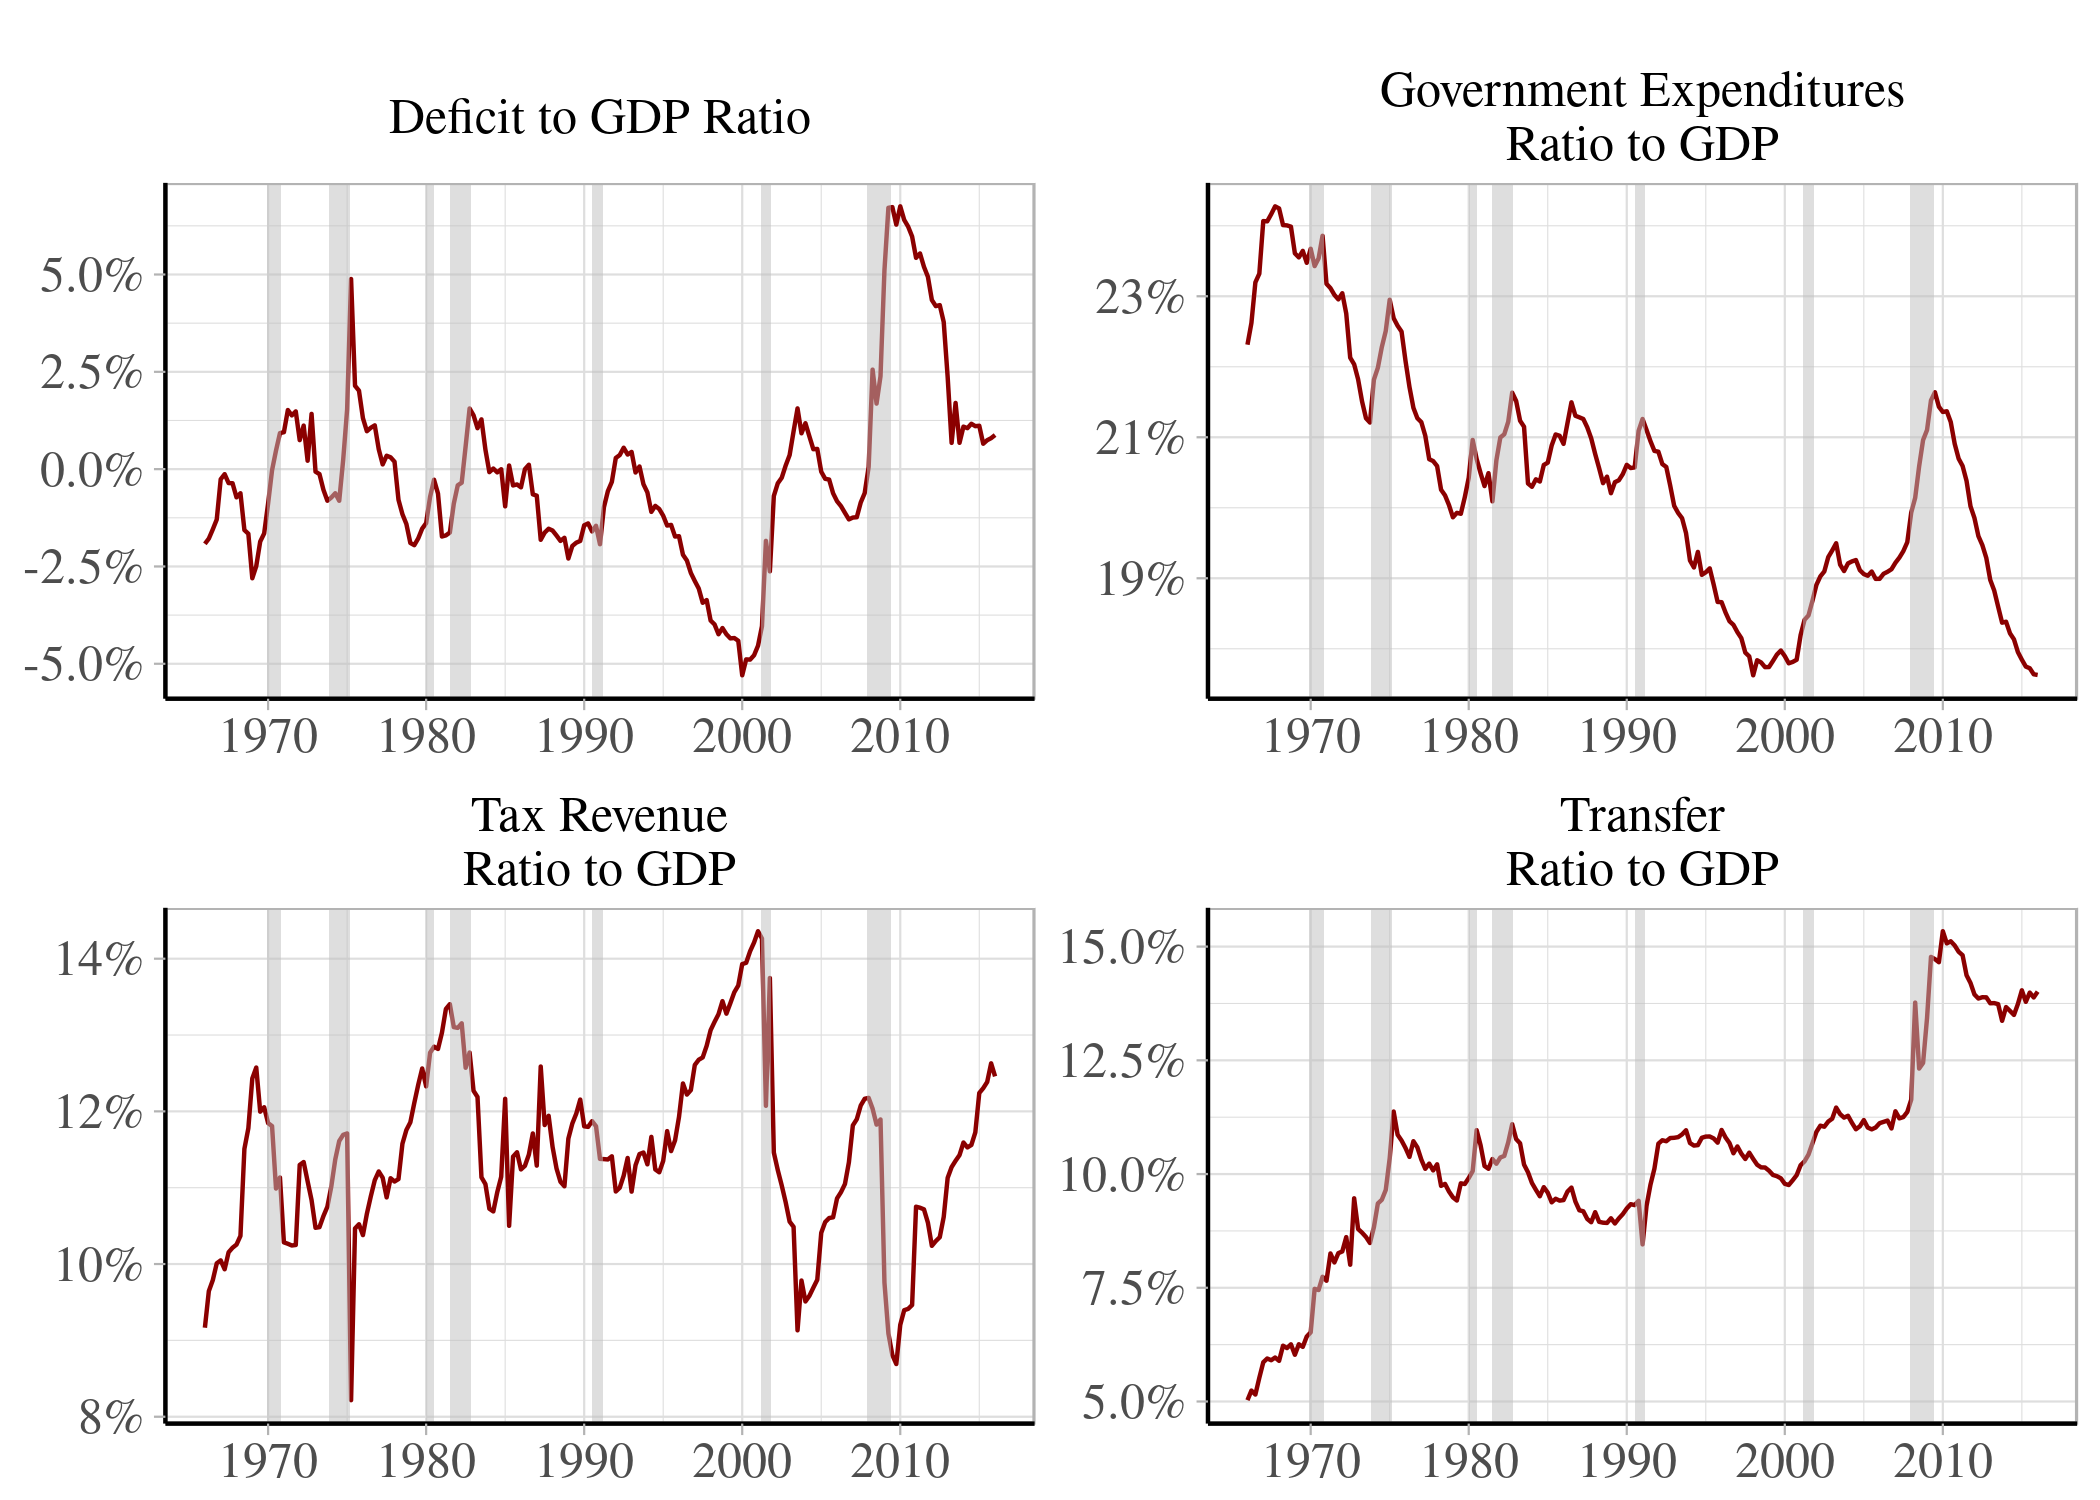
\includegraphics[align=t,width=0.95\textwidth]{./plots/data.png}
\end{frame}

\begin{comment}
\begin{frame}
  \ft{Fiscal Variables}
  \begin{tabular}{cp{1.5in}}
    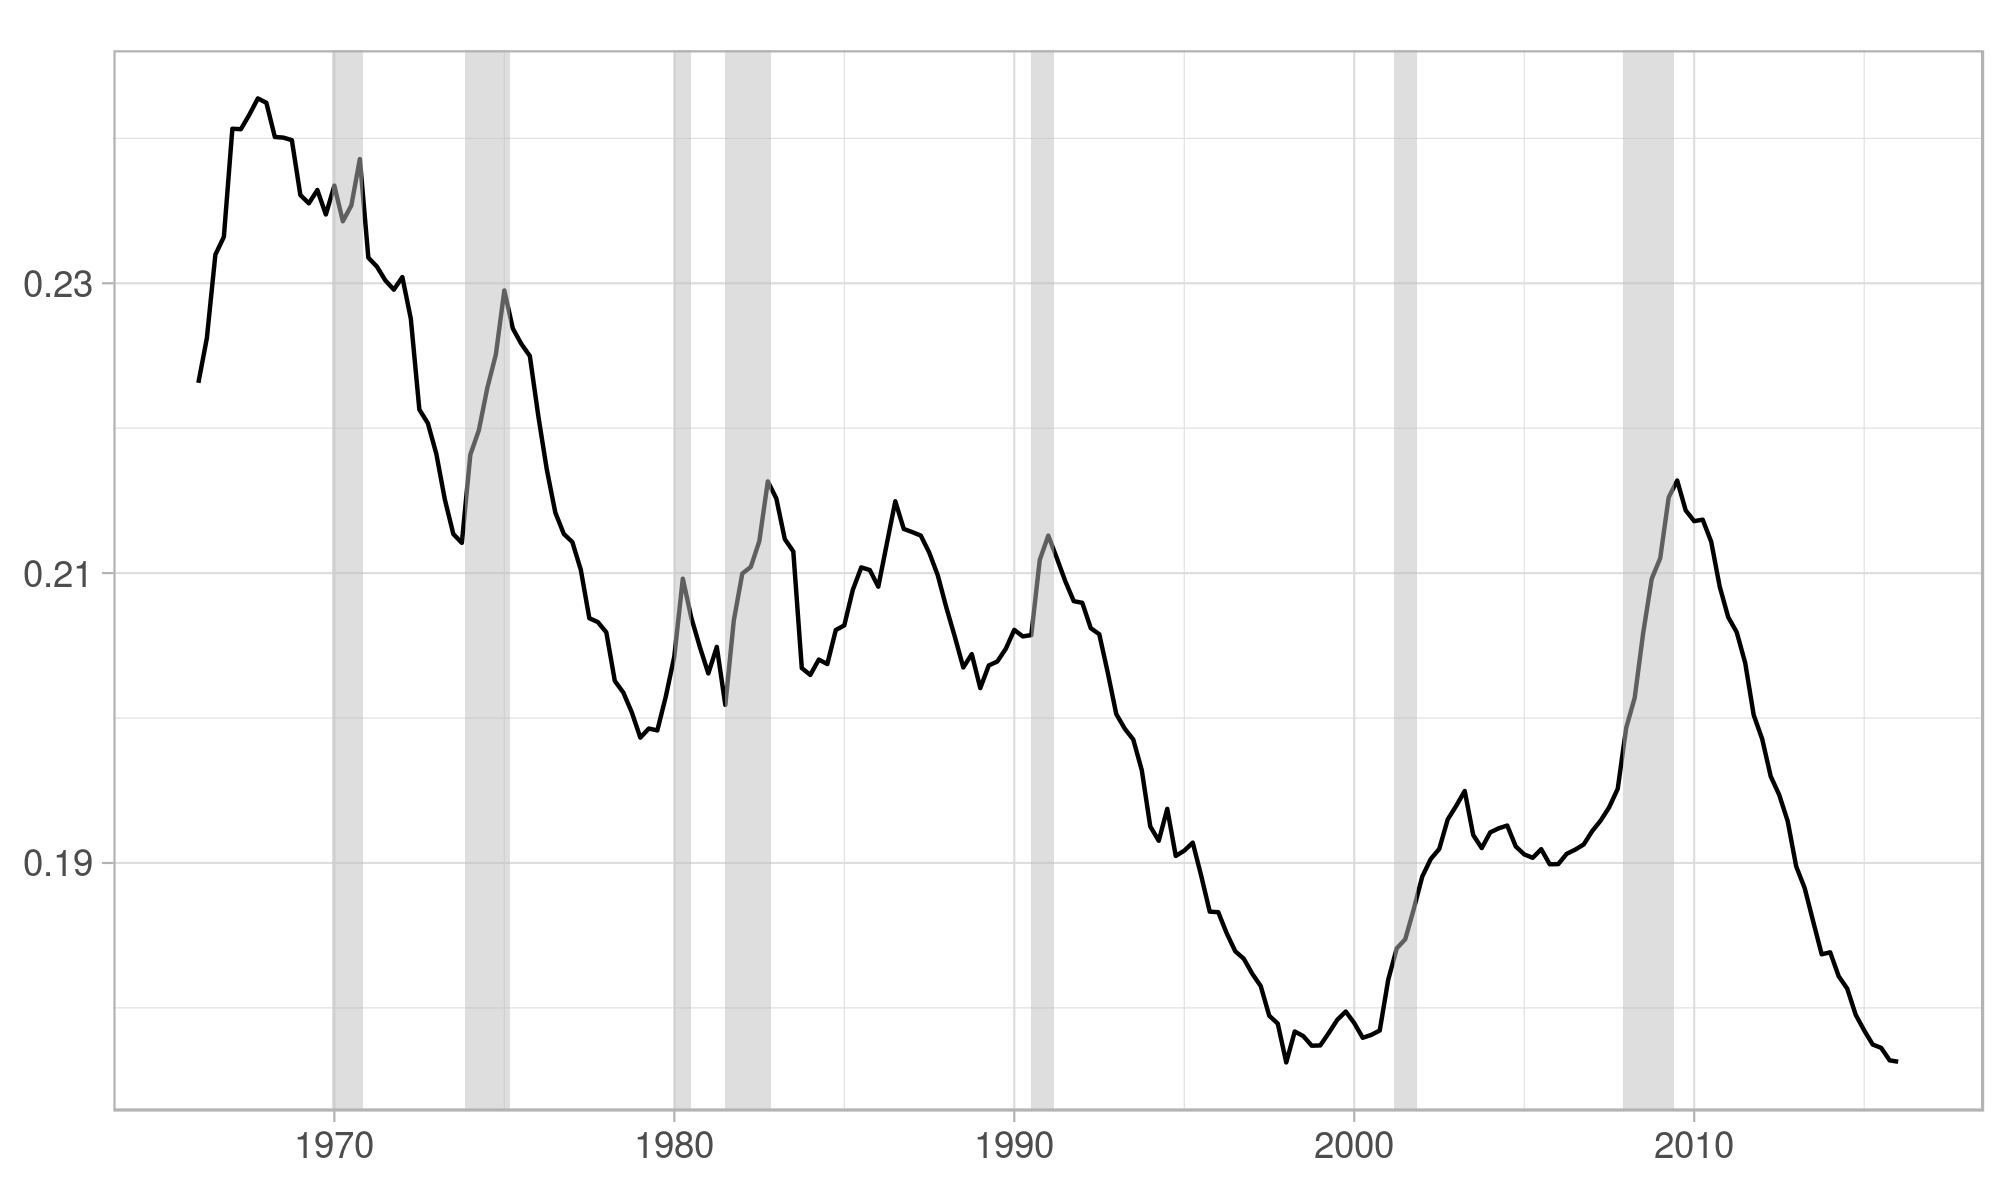
\includegraphics[align=t,height=0.41\textheight]{./gov.png} & \vspace*{2pc}Government Spending / GDP Ratio \\
    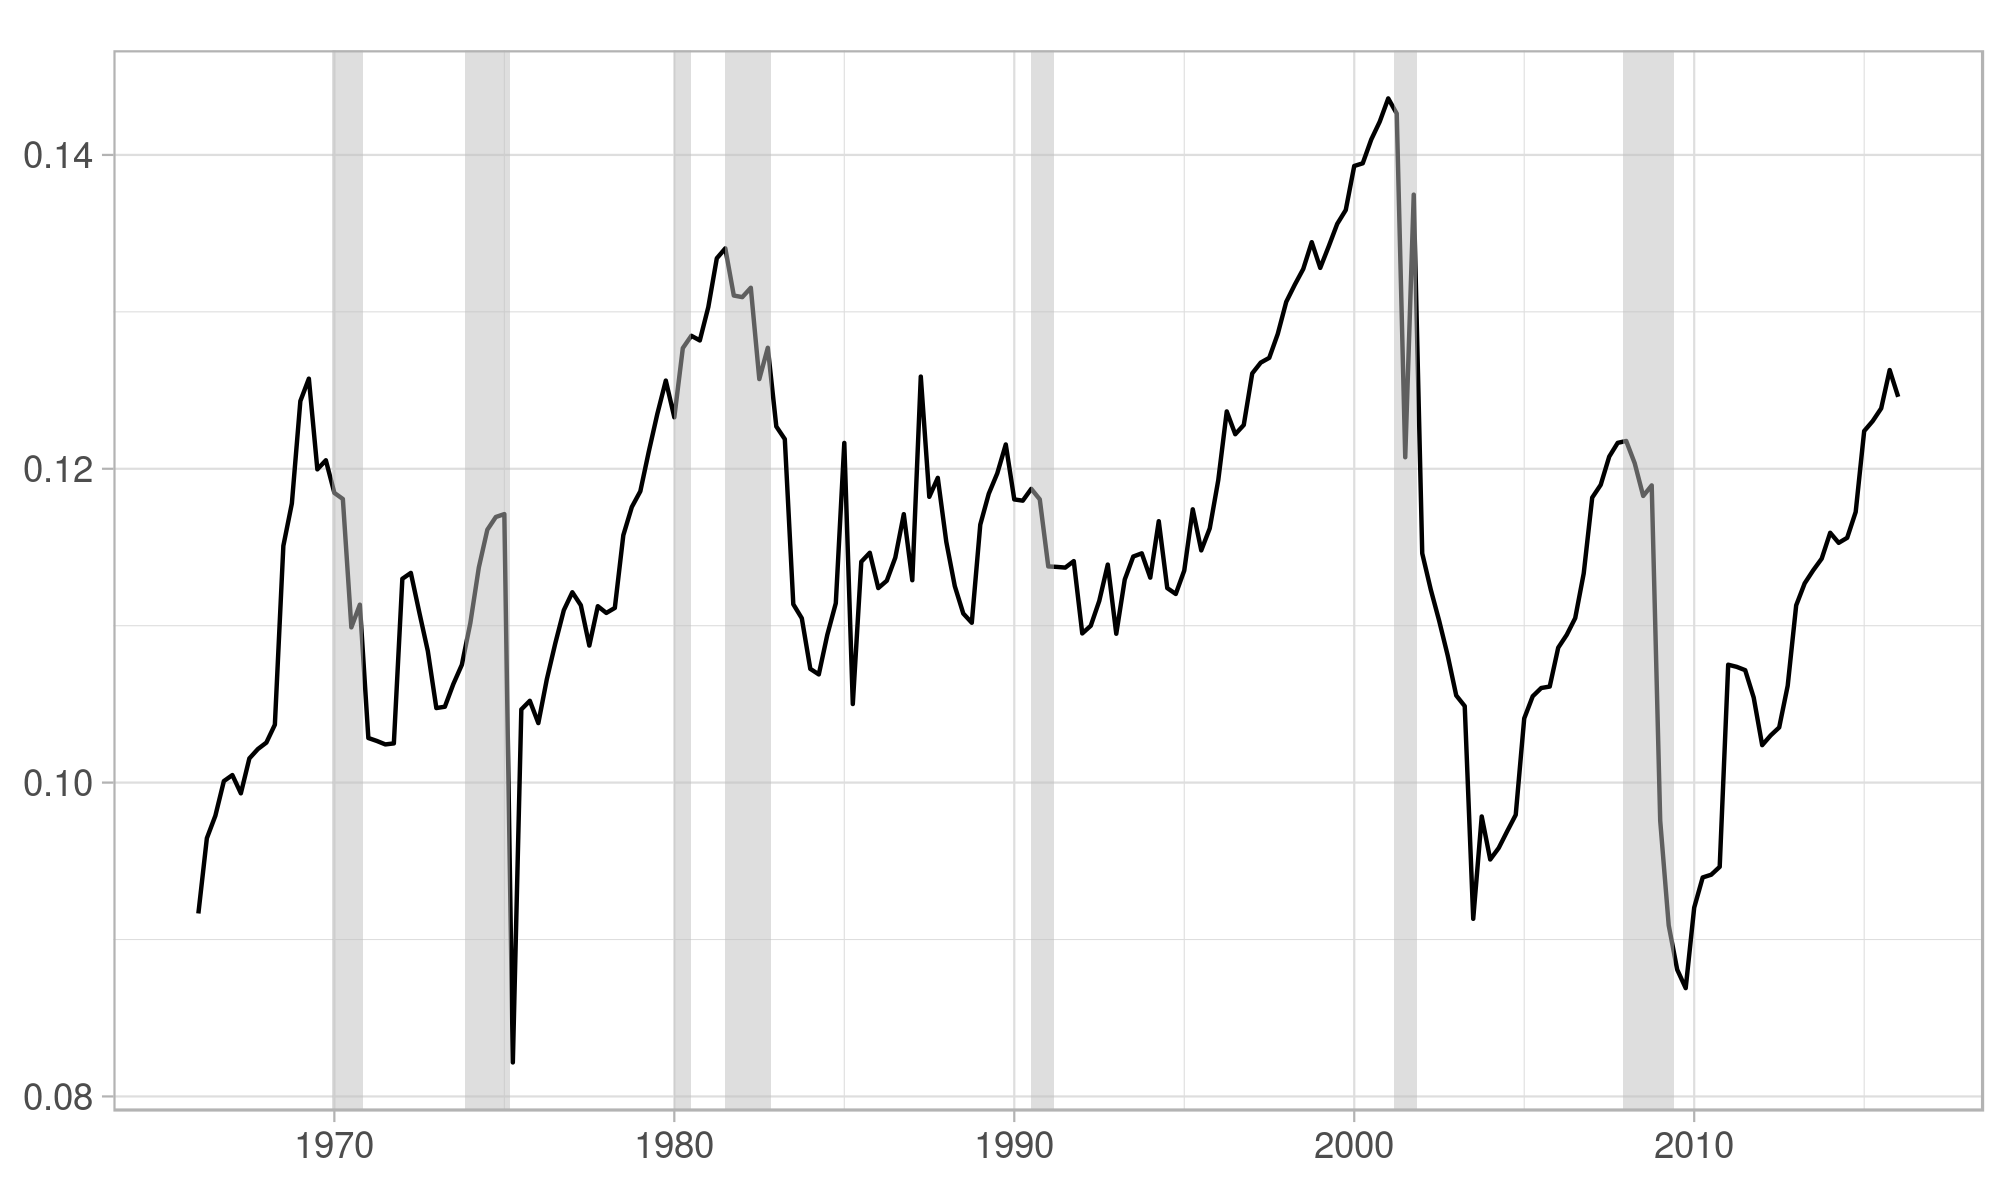
\includegraphics[align=t,height=0.41\textheight]{./tax.png} & \vspace*{2pc}Federal Tax Revenue / GDP Ratio \\
  \end{tabular}
\end{frame}

\begin{frame}
  \ft{Fiscal Variables}
  \begin{tabular}{cp{1.5in}}
    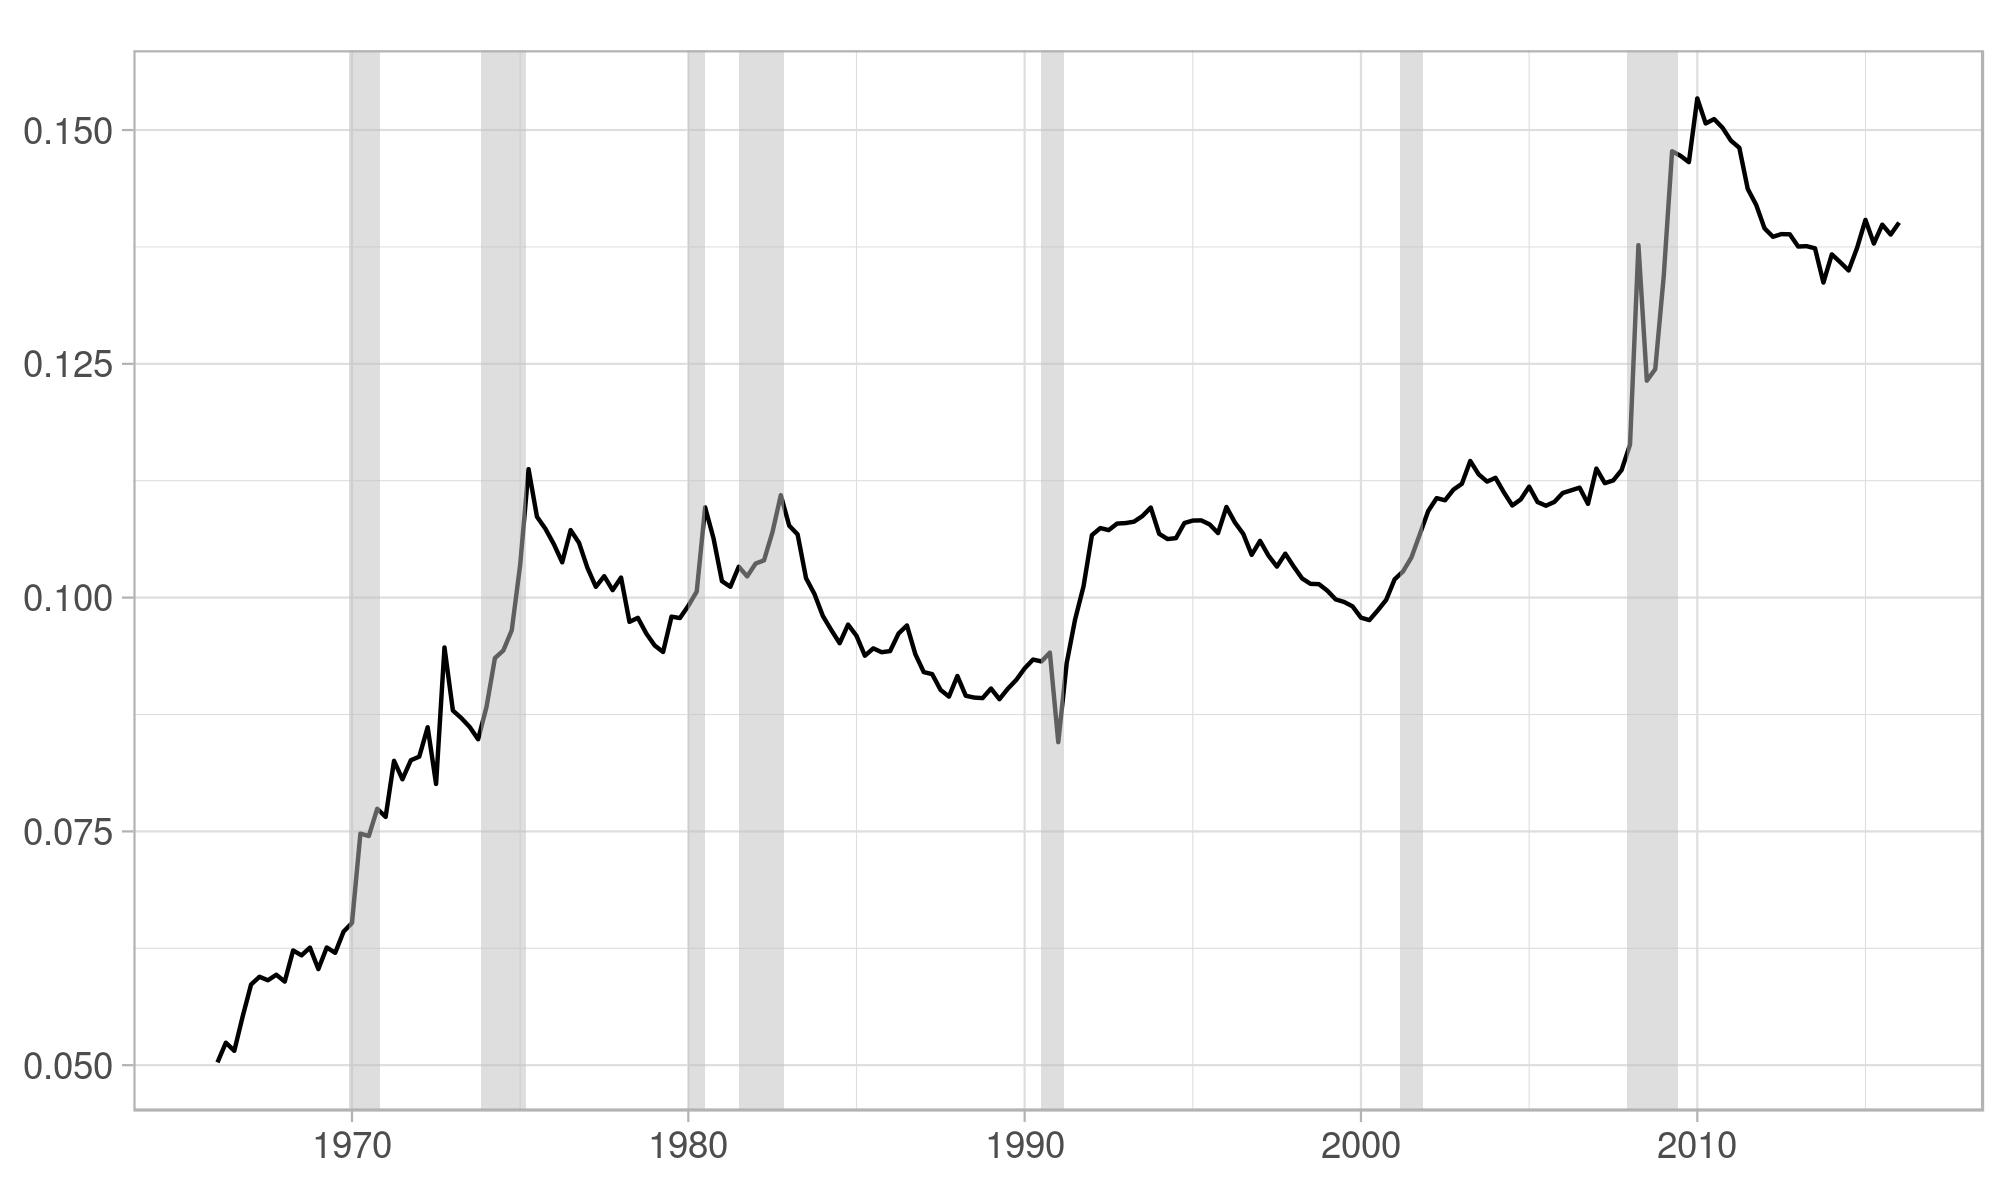
\includegraphics[align=t,height=0.41\textheight]{./transfers.png} & \vspace*{2pc}Transfers / GDP Ratio \\
    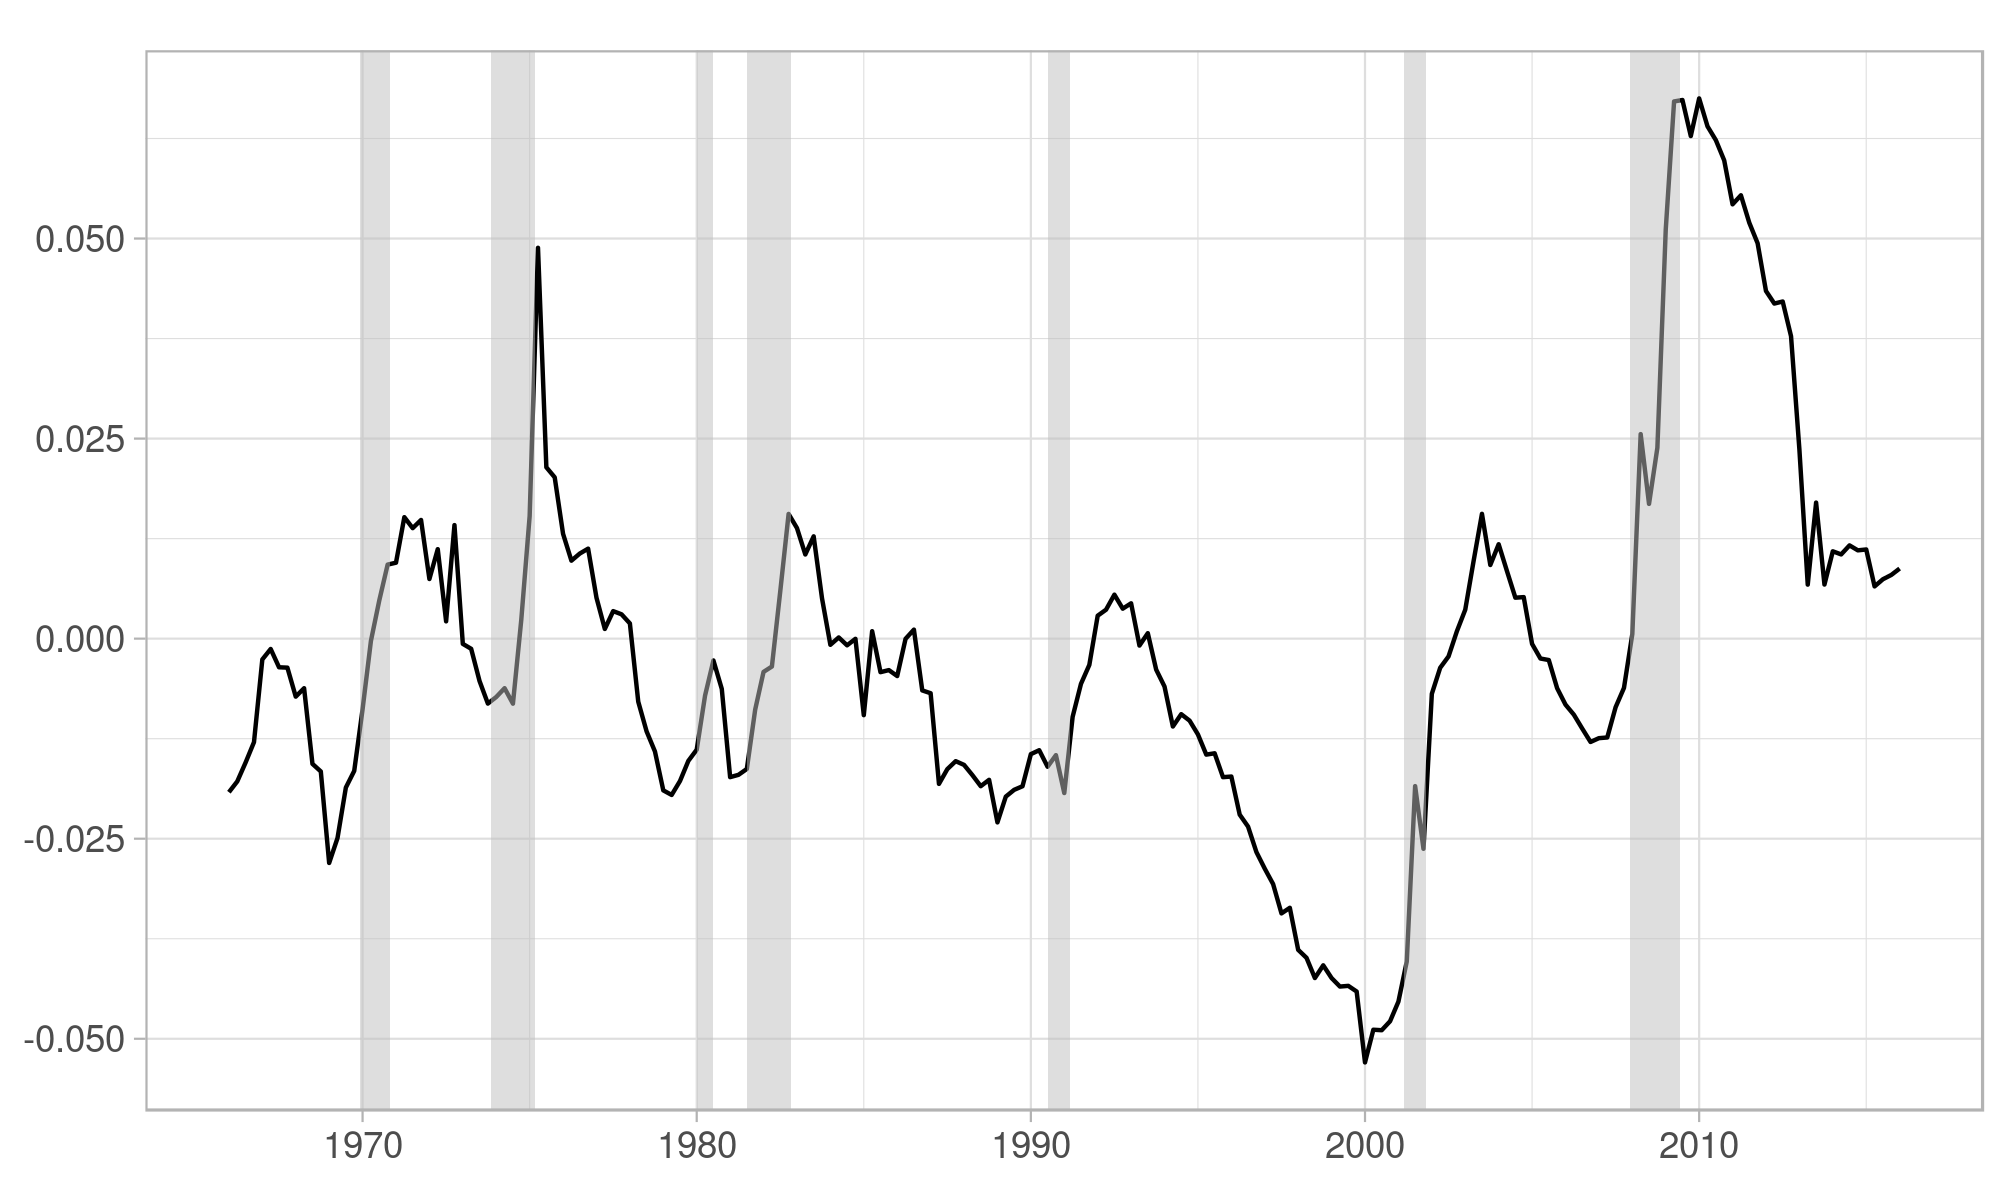
\includegraphics[align=t,height=0.41\textheight]{./deficit.png} & \vspace*{2pc}Deficit / GDP Ratio \\
  \end{tabular}
\end{frame}

\begin{frame}
  \ft{Fiscal Variables}
  \begin{tabular}{cp{1.5in}}
    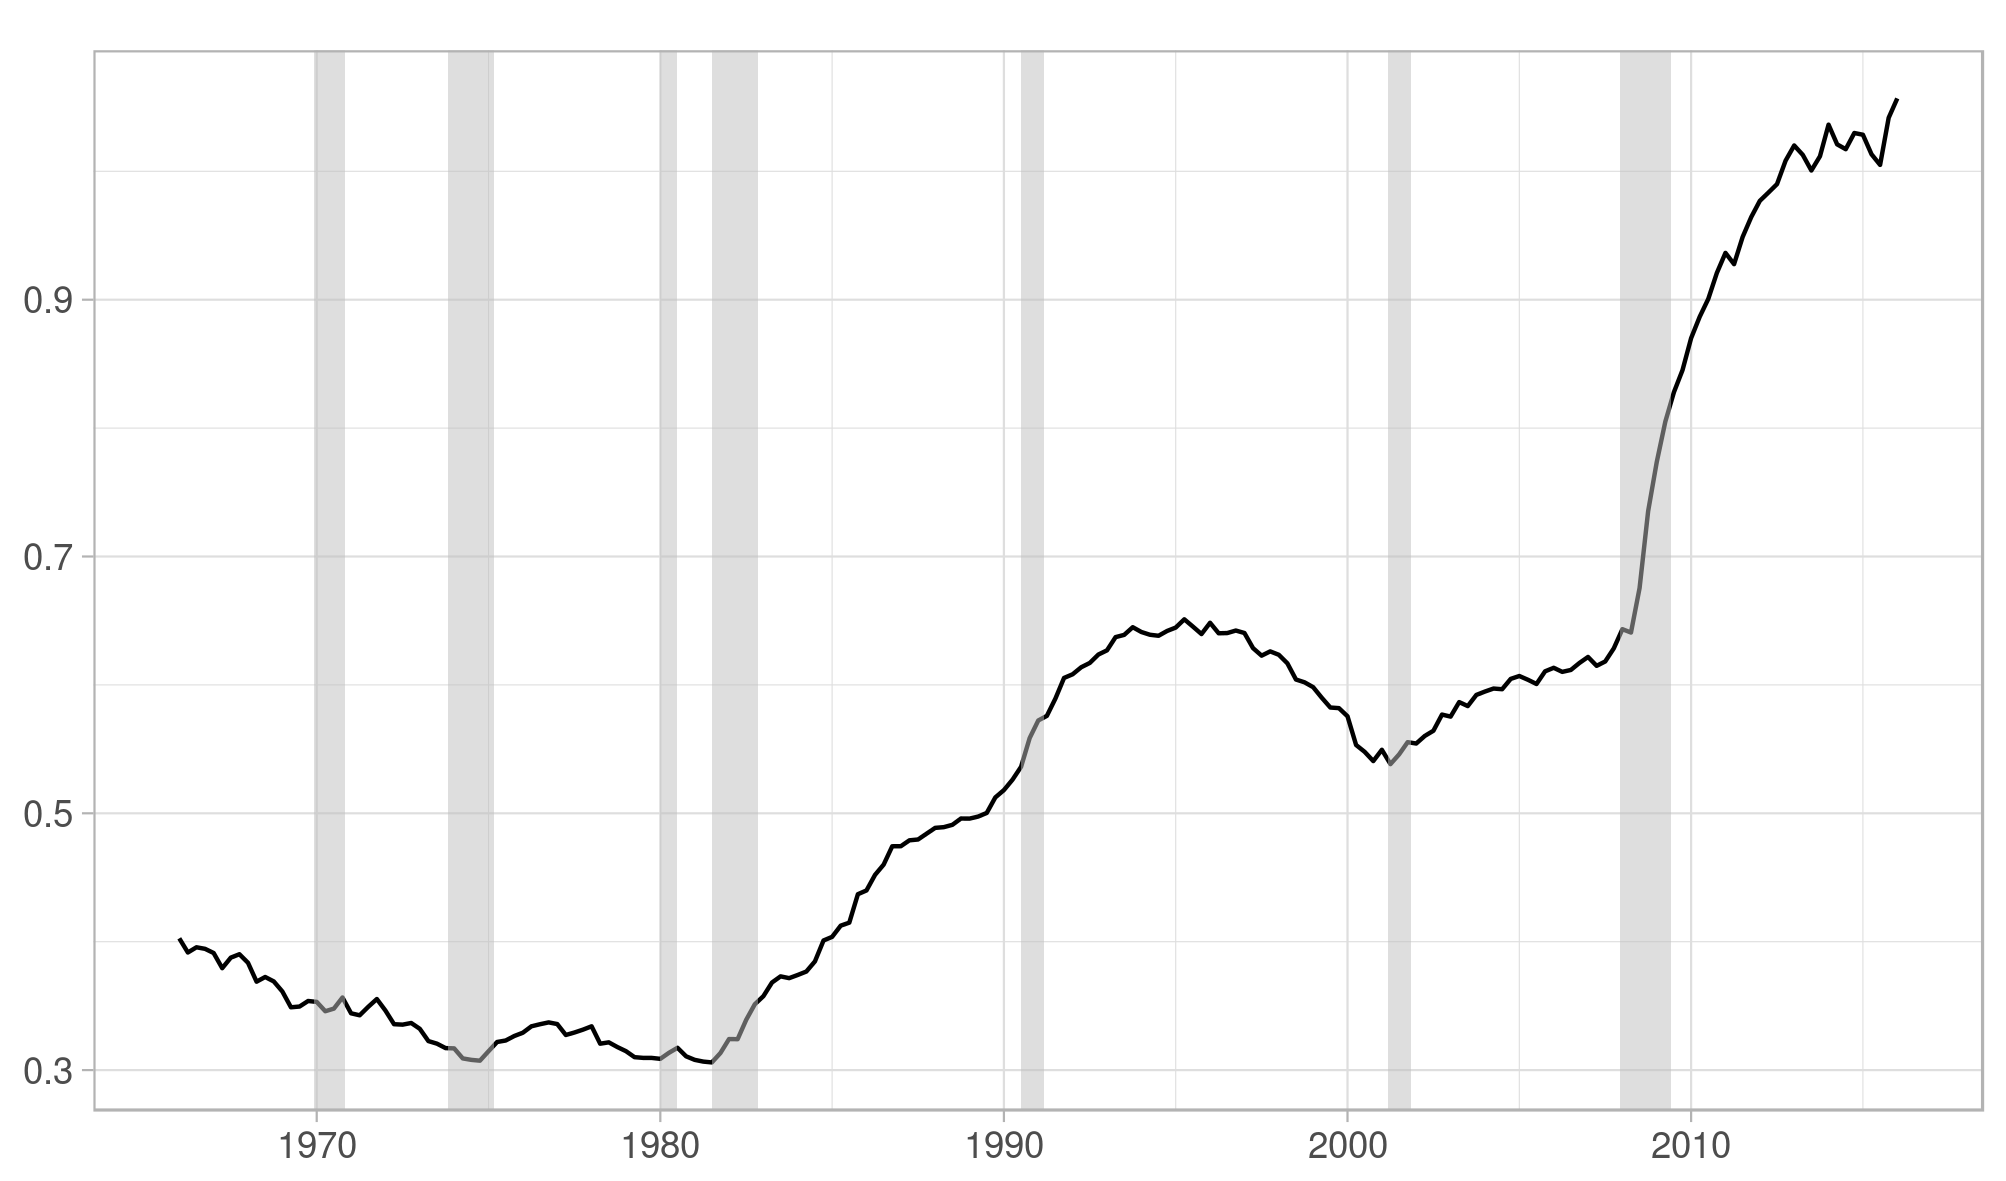
\includegraphics[align=t,height=0.41\textheight]{./debt.png} & \vspace*{2pc}Debt / GDP Ratio \\
  \end{tabular}
\end{frame}
\end{comment}




\begin{frame}
  \ft{Fiscal Policy: Government Expenditures Target}
  \small{
  \uncover<+->{
  \begin{block}{Target Policy Behavior}
    \begin{itemize}\setlength{\itemsep}{0pc}
    \item Use government expenditures to stabilize business cycle\\
      $\rightarrow$ \textbf{Decrease gov exp} in response to output gap 
    \item \textbf{Decrease government expenditures} in response to rising debt
    \end{itemize}
  \end{block}
  }
  \uncover<+->{
  \begin{block}{Structure}
    \bdm g_t^* = \bar{g}(s_t) + \psi_g(s_t) x_t + \gamma_g(s_t) \left[ b_{t-1} - \bar{b}(s_t) \right] + u_{g,t}, \edm
    \vspace*{-1.5pc}\begin{itemize}\setlength{\itemsep}{0pc}
    \item $s_t \in \{1,..,M\}$: Fiscal regime... more later
    \item $\bar{g}(s_t)$: Long-run government expenditures / GDP goal
    \item $b_{t-1}$: Lagged government debt / GDP ratio
    \item $\bar{b}(s_t)$ Long-run goal debt / GDP ratio
    \item $\psi_g(s_t) < 0$: Response to increase in output gap
    \item $\gamma_g(s_t)<0$: Response to increase in government debt
    \item $u_{g,t}$: Shock to government expenditures
    \end{itemize}
  \end{block}
  }
  }
\end{frame}

\begin{frame}
  \ft{Fiscal Policy: Tax Revenue}
  \small{
  \uncover<+->{
  \begin{block}{Target Policy Behavior}
    \begin{itemize}\setlength{\itemsep}{0pc}
    \item Use taxes to stabilize business cycle\\
      $\rightarrow$ \textbf{Increase taxes} in response to output gap 
    \item \textbf{Increase taxes} in response to rising debt
    \end{itemize}
  \end{block}
  }
  
  \uncover<+->{
    \begin{block}{Target Tax Policy}
      \bdm \tau_t^* = \bar{\tau}(s_t) + \psi_\tau(s_t) x_t + \gamma_\tau(s_t) \left[ b_{t-1} - \bar{b}(s_t) \right] + u_{\tau,t} \edm
      \vspace*{-1.4pc}\bi\setlength{\itemsep}{0pc}
      \item $\psi_\tau(s_t)>0$: Response to increase in output gap
      \item $\gamma_\tau(s_t)>0$: Response to increase in government debt
      \item $u_{\tau,t}$: Shock to tax policy
      \ei
    \end{block}
  }}
\end{frame}


\begin{frame}
  \ft{Fiscal Policy: Net Transfers}
  \small{
  
  \uncover<+->{
  \begin{block}{Target Policy Behavior}
    \begin{itemize}\setlength{\itemsep}{0pc}
    \item Use transfers to stabilize business cycle\\
      $\rightarrow$ \textbf{Decrease transfers} in response to output gap 
    \item \textbf{Decrease transfers} in response to rising debt
    \end{itemize}
  \end{block}
  }
  
  \uncover<+->{
    \begin{block}{Target Transfers Policy}
      \bdm n_t^* = \bar{n}(s_t) + \psi_n(s_t) x_t + \gamma_n(s_t) \left[ b_{t-1} - \bar{b}(s_t) \right] + u_{n,t} \edm
      \vspace*{-1.4pc}\bi\setlength{\itemsep}{0pc}
      \item $\psi_n(s_t)<0$: Response to increase in output gap
      \item $\gamma_n(s_t)<0$: Response to increase in government debt
      \item $u_{n,t}$: Shock to transfers policy
      \ei
    \end{block}
  }}
\end{frame}

\begin{frame}
  \ft{Budget Deficit}
  \uncover<+->{
    \begin{block}{Primary Budget Deficit}
      \bdm d_t = \tau_t - g_t - n_t + \tilde{d}_t \edm
      $\tilde{d}_t$: Deficit residual\newline
      \hspace*{1.2pc}(Other expenditure or revenue items I did not include)
    \end{block}
  }
  \uncover<+->{
    \begin{block}{Deficit Residual Behavior}
      \bdm d_t^* =\bar{\tilde{d}}(s_t) + \psi_d(s_t) x_t + \gamma_d(s_t) \left[ b_{t-1} - \bar{b}(s_t) \right] + u_{d,t} \edm
    \end{block}
  }
\end{frame}


\begin{frame}
  \ft{Variances}
  
  \uncover<+->{
  \begin{block}{Regime-dependent variances for fiscal shocks}
    \begin{tabular}{ll}
      $\sigma_g^2(s_t)$: Var(shock to gov exp) & $\sigma_n^2(s_t)$: Var(shock to transfers) \\
      $\sigma_\tau(s_t)$: Var(shock to taxes) & $\sigma_d^2(s_t)$: Var(shock to deficits) \end{tabular}
  \end{block}}

  \uncover<+->{
  \begin{block}{Correlations of fiscal shocks}
    \begin{itemize}
    \item Fiscal policy decisions are dependent on one another.
    \item Consider all possible correlations:\\
      \hspace{2pc} $\varrho_{g,\tau}$, $\varrho_{\tau,n}$, $\varrho_{g,n}$, $\varrho_{\tau,d}$, $\varrho_{g,d}$, $\varrho_{n,d}$
    \end{itemize}
  \end{block}
  }
\end{frame}

\begin{frame}
  \ft{Three Sources for Regime Switching}
  \begin{footnotesize}
    \uncover<+->{\begin{block}{Long-run Debt Target Regimes}
    \setbeamertemplate{enumerate items}[default]
    \begin{enumerate}[{Regime} A:]
      \setcounter{enumi}{11}
      \item \textit{Low} long-run target for debt/GDP (low value for  $\bar{b}(s_t)$)
      \setcounter{enumi}{7}
      \item \textit{High} long-run target for debt/GDP (high value for  $\bar{b}(s_t)$)
    \end{enumerate}
  \end{block}}

  \uncover<+->{
    \begin{block}{Fiscal Financing}
      \bi
      \item Targets for fiscal components: $\bar{g}(s_t)$, $\bar{\tau}(s_t)$, $\bar{n}(s_t)$, $\bar{d}(s_t)$
      \item Behavior toward output gap and debt: $\psi_f(s_t)$ and $\gamma_f(s_t)$, for $f \in \{g,\tau,n,\tilde{d}\}$
      \ei
      \setbeamertemplate{enumerate items}[default]
      \vspace*{-0.5pc}\begin{enumerate}[{Regime} A:]
      \item Fiscal behavior A
      \item Fiscal behavior B
      \end{enumerate}
    \end{block}
  }

  \uncover<+->{
    \begin{block}{Fiscal Volatility}
      Two regimes to determine variances, $\sigma_g^2(s_t)$, $\sigma_\tau^2(s_t)$, $\sigma_n^2(s_t)$, and $\sigma_d^2(s_t)$:
          \setbeamertemplate{enumerate items}[default]
          \begin{enumerate}[{Regime} A:]
        \setcounter{enumi}{18}
        \item \textit{Stable}, relatively smaller variances
        \setcounter{enumi}{21}
        \item \textit{Volatile}, relatively larger variances 
      \end{enumerate}
    \end{block}
  }
  \end{footnotesize}
  
\end{frame}

\begin{frame}
  \ft{Regime Switching Procedure}
  \begin{footnotesize}
  \uncover<+-> {
  \begin{block}{Markov regime switching}
    Regime switches randomly, each source \textbf{independently} of other sources
    \bi
    \item $p_L=P(s_t=L | s_{t-1}=L)$ be prob policy remains in reg L
    \item $p_H=P(s_t=H | s_{t-1}=H)$ be prob policy remains in reg H
    \item $p_A=P(s_t=A | s_{t-1}=A)$ be prob policy remains in reg A
    \item $p_A=P(s_t=B | s_{t-1}=B)$ be prob policy remains in reg B
    \item $p_A=P(s_t=S | s_{t-1}=S)$ be prob policy remains in reg S
    \item $p_A=P(s_t=V | s_{t-1}=V)$ be prob policy remains in reg V
    \ei
  \end{block}}

  \uncover<+->{\begin{block}{Rich Set of Regime-Switching Possibilities} 
      \bi
      \item Changes in priorities for taxes, transfers, spending, \textit{without adjusting long-run targets for debt/GDP}
      \item Changes in debt-targets, \textit{without adjusting purposes and priorities for fiscal components}
      \item Changes in volatility of fiscal outcomes, \textit{without changing goals or purposes}
      \ei
  \end{block}}
  \end{footnotesize}
\end{frame}


\begin{frame}
  \ft{Data}
  \begin{footnotesize}

  \uncover<+->{\begin{block}{Fiscal policy variables}
  \be
  \item Nominal government expenditures: NIPA Table 1.1.5, Line 22
  \item Tax revenue: NIPA Table 3.2, Line 3
  \item Net transfers: Federal current transfer pmts - receipts
    \bi \item NIPA Table 3.2, (Line 25 - Line 18) \ei
  \item Primary budget deficit:
    \bi \item (-) net federal government saving - federal interest payments
    \item NIPA Table 3.2, Line 36 - Line 32 \ei
  \item Government debt: Federal debt held by the public (U.S. Dept of Treasury)
  \ee
  \end{block}}

  \uncover<+->{\begin{block}{Remaining variables}
    \be
    \setcounter{enumi}{5}
    \item Nominal GDP: NIPA Table 1.1.5, Line 1
    \item Output gap: Difference between NGDP and potential GDP 
    \item Inflation: Growth GDP implicit price deflator (NIPA Table 1.1.9, Line 1)
    \item Interest rate: Federal funds rate
      \ee
  \end{block}}
  \end{footnotesize}
\end{frame}

\begin{frame}
  \ft{Results: Government Expenditures Behavior}
  \small{
    \uncover<+->{\begin{block}{Posterior Parameter Distributions Under Regimes A \& B}
      \setlength{\tabcolsep}{2pt}
      \begin{tabular}{clcccc}
        & & \multicolumn{2}{c}{Fiscal Regime A} & \multicolumn{2}{c}{Fiscal Regime B} \\ 
        Param. & Description & Median & 90\% Bounds & Median & 90\% Bounds \\ \hline
        \hl{2}{$\bar{g}$} & \hl{2}{Long-run gov target} & \hl{2}{0.19} & \hl{2}{(0.18, 0.20)} & \hl{2}{0.31} & \hl{2}{(0.29, 0.32)} \\ [0.2pc]
        \hl{3}{$\psi_{g}$} & \hl{3}{Resp to output gap} & \hl{3}{-0.32} & \hl{3}{(-0.38, -0.28)} & \hl{3}{-0.43} & \hl{3}{(-0.45, -0.39)} \\ [0.2pc]
        \hl{4}{$\gamma_{g}$} & \hl{4}{Resp to debt} & \hl{4}{-0.55} & \hl{4}{(-0.61, -0.49)} & \hl{4}{-0.44} & \hl{4}{(-0.50, -0.40)} \\ \hline
      \end{tabular}
    \end{block}}

    \uncover<+->{\begin{block}{Description}
      \bi
      \item<2> \hl{2}{Fiscal Regime A has \textbf{lower long-run} government expenditures}
      \item<3> \hl{3}{Fiscal regime A has gov exp \textbf{less responsive to output gap}}
      \item<4> \hl{4}{Fiscal regime A has gov exp \textbf{more responsive to debt}}
      \ei
    \end{block}
    }
  }
\end{frame}

\begin{frame}
  \ft{Results: Tax Behavior}
  \small{
    \uncover<+->{\begin{block}{Posterior Parameter Distributions Under Regimes A \& B}
      \setlength{\tabcolsep}{2pt}
      \begin{tabular}{clcccc}
        & & \multicolumn{2}{c}{Fiscal Regime A} & \multicolumn{2}{c}{Fiscal Regime B} \\ 
        Param. & Description & Median & 90\% Bounds & Median & 90\% Bounds \\ \hline
        \hl{2}{$\bar{\tau}$} & \hl{2}{Long-run tax target} & \hl{2}{0.14} & \hl{2}{(0.13, 0.14)} & \hl{2}{0.28} & \hl{2}{(0.25, 0.29)} \\ [0.2pc]
        \hl{3}{$\psi_{\tau}$} & \hl{3}{Resp to output gap} & \hl{3}{0.69} & \hl{3}{(0.68, 0.72)} & \hl{3}{0.47} & \hl{3}{(0.44, 0.55)} \\ [0.2pc]
        \hl{4}{$\gamma_{\tau}$} & \hl{4}{Resp to debt} & \hl{4}{0.25} & \hl{4}{(0.23, 0.29)} & \hl{4}{0.34} & \hl{4}{(0.26, 0.44)} \\ \hline
      \end{tabular}
    \end{block}}

    \uncover<+->{\begin{block}{Description}
      \bi
      \item<2> \hl{2}{Fiscal Regime A has \textbf{lower long-run} tax target}
      \item<3> \hl{3}{Fiscal regime A has taxes \textbf{more responsive to output gap}}
      \item<4> \hl{4}{Fiscal regime A has taxes \textbf{less responsive to debt}}
      \ei
    \end{block}
    }
  }
\end{frame}


\begin{frame}
  \ft{Results: Transfers Behavior}
  \small{
    \uncover<+->{\begin{block}{Posterior Parameter Distributions Under Regimes A \& B}
      \setlength{\tabcolsep}{2pt}
      \begin{tabular}{clcccc}
        & & \multicolumn{2}{c}{Fiscal Regime A} & \multicolumn{2}{c}{Fiscal Regime B} \\ 
        Param. & Description & Median & 90\% Bounds & Median & 90\% Bounds \\ \hline
        \hl{2}{$\bar{n}$} & \hl{2}{Long-run transfers} & \hl{2}{0.11} & \hl{2}{(0.10, 0.13)} & \hl{2}{0.18} & \hl{2}{(0.17, 0.20)} \\ [0.2pc]
        \hl{3}{$\psi_{n}$} & \hl{3}{Resp to output gap} & \hl{3}{-0.46} & \hl{3}{(-0.49, -0.41)} & \hl{3}{-0.50} & \hl{3}{(-0.54, -0.43)} \\ [0.2pc]
        \hl{4}{$\gamma_{n}$} & \hl{4}{Resp to debt} & \hl{4}{-0.33} & \hl{4}{(-0.37, -0.26)} & \hl{4}{-0.51} & \hl{4}{(-0.55, -0.47)} \\ \hline
      \end{tabular}
    \end{block}}

    \uncover<+->{\begin{block}{Description}
      \bi
      \item<2> \hl{2}{Fiscal Regime A has \textbf{lower long-run} transfers}
      \item<3> \hl{3}{Regimes are \textbf{not different on responsiveness to output gap}}
      \item<4> \hl{4}{Fiscal regime A has transfers \textbf{less responsive to debt}}
      \ei
    \end{block}
    }
  }
\end{frame}



\begin{frame}
  \ft{Results: Debt Regimes}
  \small{
    \uncover<+->{\begin{block}{Posterior Parameter Distributions Under Low \& High Debt Regimes}
      \setlength{\tabcolsep}{2pt}
      \begin{tabular}{clcccc}
        & & \multicolumn{2}{c}{Low Debt Regime} & \multicolumn{2}{c}{High Debt Regime} \\ 
        Param. & Description & Median & 90\% Bounds & Median & 90\% Bounds \\ \hline
        $\bar{b}$ & Debt/GDP target & 0.37 & (0.34, 0.39) & 0.60 & (0.55, 0.64) \\ \hline
      \end{tabular}
    \end{block}}

    \uncover<.->{\begin{block}{Debt Regimes}
      Low debt regime $\approx$ 37\% of GDP\\
      High debt regime $\approx$ 60\% of GDP
    \end{block}
    }
  }
\end{frame}

\begin{frame}
  \ft{Results: Volatility Regimes}
  \small{
    \uncover<+->{\begin{block}{Posterior Parameter Distributions Under Stable and Volatile Regimes}
       \setlength{\tabcolsep}{4pt}
       \begin{tabular}{clcccc}
        & & \multicolumn{2}{c}{Stable Regime} & \multicolumn{2}{c}{Volatile Regime} \\ 
        Param. & Description & Median & 90\% Bounds & Median & 90\% Bounds \\ \hline
        $\sigma_{g}$ & Gov stdev & 0.10 & (0.09, 0.11) & 0.19 & (0.17, 0.22) \\ 
        $\sigma_{\tau}$ & Tax stdev & 0.10 & (0.10, 0.11) & 0.29 & (0.28, 0.30) \\ 
        $\sigma_{n}$ & Transfers stdev & 0.06 & (0.06, 0.08) & 0.22 & (0.19, 0.26) \\ 
        $\sigma_{d}$ & Deficit stdev & 0.08 & (0.08, 0.10) & 0.20 & (0.19, 0.22) \\ \hline
      \end{tabular}
    \end{block}}
  }
  \ \\
  \textcolor{BrickRed}{All standard deviations are larger in volatile regime,\\\textbf{most more than double}.}
\end{frame}

\begin{frame}
  \ft{Timing of Fiscal Regimes}
  \begin{center}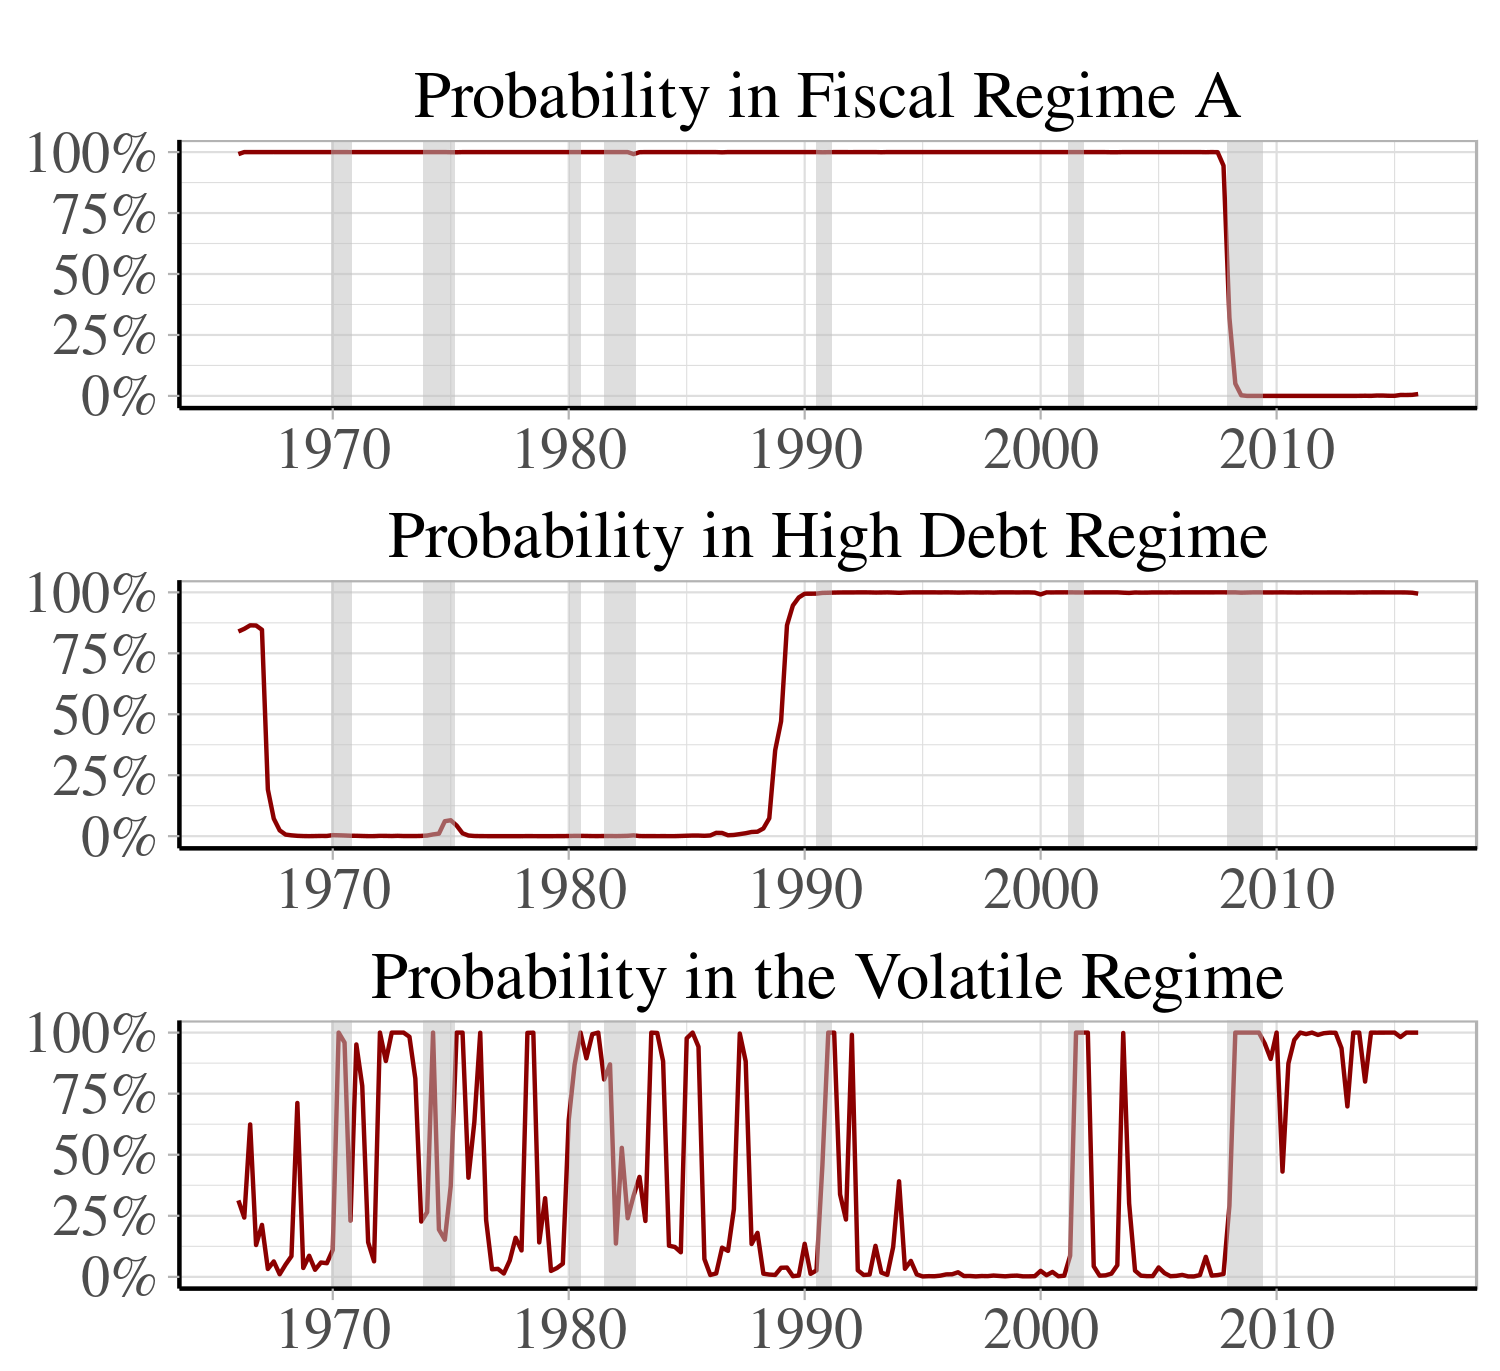
\includegraphics[align=t,height=0.85\textheight]{./plots/regimes.png}\end{center}
\end{frame}

\begin{frame}
  \ft{Conclusions}
  \bi
  \item<+-> Evidence of switching in all three dimensions.
  \item<+-> Switch from low-debt to high-debt regime in 1989.
  \item<+-> Single, permanent, switch in fiscal policy behavior in 2008.
    \bi
    \item Government expenditures playing larger role in macroeconomic stabilization, smaller role in balancing budget.
    \item Taxes play smaller role in macroeconomic stabilization, larger role in balancing budget.
      \ei
  \item<+-> Many switches from stable to volatile fiscal regimes, usually around and following recessions.
  \ei   
\end{frame}


\end{document}

